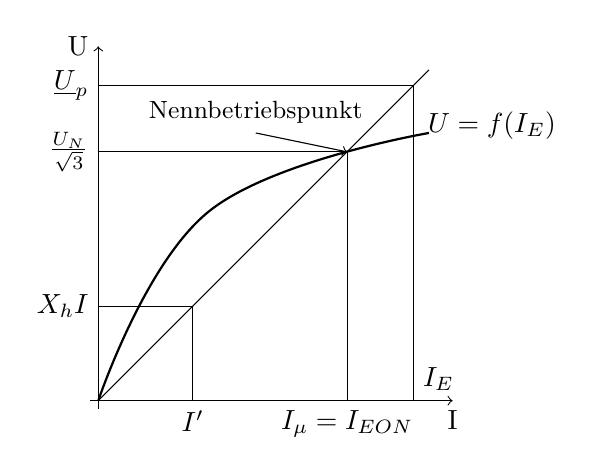
\begin{tikzpicture}
 	\draw[->] (-0.1,0) -- +(4.6,0) node[below] {I};
 	\draw[->] (0,-0.1) -- +(0,4.6) node[left]{U};
 	\draw (0,0) -- +(4.2,4.2);
	\draw[thick]  plot[smooth, tension=.7] coordinates {(0,0) (1.4,2.4) (4.2,3.4)};
	\draw (5,3.5) node[] {$U = f(I_E)$};
	
	\draw (1.2,0) node[below] {$I'$}
		-- ++(0,1.2) 
		-- ++(-1.2,0) node[left] {$X_h I$};
	\draw (3.16,0) node[below] {$I_\mu = I_{EON}$}
		-- ++(0,3.16) 
		-- ++(-3.16,0) node[left] {$\frac{U_N}{\sqrt{3}}$};
	\draw (4,0) node[above right] {$I_E$}
		-- ++(0,4) 
		-- ++(-4,0) node[left] {$\underline{U}_p$};
	\draw[<-] (3.16,3.16) -- (2,3.4) node[above]{\small{Nennbetriebspunkt}};
\end{tikzpicture}